% Options for packages loaded elsewhere
\PassOptionsToPackage{unicode}{hyperref}
\PassOptionsToPackage{hyphens}{url}
\PassOptionsToPackage{dvipsnames,svgnames,x11names}{xcolor}
%
\documentclass[
  letterpaper,
  DIV=11,
  numbers=noendperiod]{scrartcl}

\usepackage{amsmath,amssymb}
\usepackage{lmodern}
\usepackage{iftex}
\ifPDFTeX
  \usepackage[T1]{fontenc}
  \usepackage[utf8]{inputenc}
  \usepackage{textcomp} % provide euro and other symbols
\else % if luatex or xetex
  \usepackage{unicode-math}
  \defaultfontfeatures{Scale=MatchLowercase}
  \defaultfontfeatures[\rmfamily]{Ligatures=TeX,Scale=1}
\fi
% Use upquote if available, for straight quotes in verbatim environments
\IfFileExists{upquote.sty}{\usepackage{upquote}}{}
\IfFileExists{microtype.sty}{% use microtype if available
  \usepackage[]{microtype}
  \UseMicrotypeSet[protrusion]{basicmath} % disable protrusion for tt fonts
}{}
\usepackage{xcolor}
\usepackage[top=20mm,left=18mm,right=18mm,heightrounded]{geometry}
\setlength{\emergencystretch}{3em} % prevent overfull lines
\setcounter{secnumdepth}{5}
% Make \paragraph and \subparagraph free-standing
\ifx\paragraph\undefined\else
  \let\oldparagraph\paragraph
  \renewcommand{\paragraph}[1]{\oldparagraph{#1}\mbox{}}
\fi
\ifx\subparagraph\undefined\else
  \let\oldsubparagraph\subparagraph
  \renewcommand{\subparagraph}[1]{\oldsubparagraph{#1}\mbox{}}
\fi


\providecommand{\tightlist}{%
  \setlength{\itemsep}{0pt}\setlength{\parskip}{0pt}}\usepackage{longtable,booktabs,array}
\usepackage{calc} % for calculating minipage widths
% Correct order of tables after \paragraph or \subparagraph
\usepackage{etoolbox}
\makeatletter
\patchcmd\longtable{\par}{\if@noskipsec\mbox{}\fi\par}{}{}
\makeatother
% Allow footnotes in longtable head/foot
\IfFileExists{footnotehyper.sty}{\usepackage{footnotehyper}}{\usepackage{footnote}}
\makesavenoteenv{longtable}
\usepackage{graphicx}
\makeatletter
\def\maxwidth{\ifdim\Gin@nat@width>\linewidth\linewidth\else\Gin@nat@width\fi}
\def\maxheight{\ifdim\Gin@nat@height>\textheight\textheight\else\Gin@nat@height\fi}
\makeatother
% Scale images if necessary, so that they will not overflow the page
% margins by default, and it is still possible to overwrite the defaults
% using explicit options in \includegraphics[width, height, ...]{}
\setkeys{Gin}{width=\maxwidth,height=\maxheight,keepaspectratio}
% Set default figure placement to htbp
\makeatletter
\def\fps@figure{htbp}
\makeatother

\usepackage{float}
\KOMAoption{captions}{tableheading}
\makeatletter
\makeatother
\makeatletter
\makeatother
\makeatletter
\@ifpackageloaded{caption}{}{\usepackage{caption}}
\AtBeginDocument{%
\ifdefined\contentsname
  \renewcommand*\contentsname{Índice}
\else
  \newcommand\contentsname{Índice}
\fi
\ifdefined\listfigurename
  \renewcommand*\listfigurename{Lista de Figuras}
\else
  \newcommand\listfigurename{Lista de Figuras}
\fi
\ifdefined\listtablename
  \renewcommand*\listtablename{Lista de Tabelas}
\else
  \newcommand\listtablename{Lista de Tabelas}
\fi
\ifdefined\figurename
  \renewcommand*\figurename{Figura}
\else
  \newcommand\figurename{Figura}
\fi
\ifdefined\tablename
  \renewcommand*\tablename{Tabela}
\else
  \newcommand\tablename{Tabela}
\fi
}
\@ifpackageloaded{float}{}{\usepackage{float}}
\floatstyle{ruled}
\@ifundefined{c@chapter}{\newfloat{codelisting}{h}{lop}}{\newfloat{codelisting}{h}{lop}[chapter]}
\floatname{codelisting}{Listagem}
\newcommand*\listoflistings{\listof{codelisting}{Lista de Listagens}}
\makeatother
\makeatletter
\@ifpackageloaded{caption}{}{\usepackage{caption}}
\@ifpackageloaded{subcaption}{}{\usepackage{subcaption}}
\makeatother
\makeatletter
\@ifpackageloaded{tcolorbox}{}{\usepackage[many]{tcolorbox}}
\makeatother
\makeatletter
\@ifundefined{shadecolor}{\definecolor{shadecolor}{rgb}{.97, .97, .97}}
\makeatother
\makeatletter
\makeatother
\ifLuaTeX
\usepackage[bidi=basic]{babel}
\else
\usepackage[bidi=default]{babel}
\fi
\babelprovide[main,import]{portuguese}
% get rid of language-specific shorthands (see #6817):
\let\LanguageShortHands\languageshorthands
\def\languageshorthands#1{}
\ifLuaTeX
  \usepackage{selnolig}  % disable illegal ligatures
\fi
\IfFileExists{bookmark.sty}{\usepackage{bookmark}}{\usepackage{hyperref}}
\IfFileExists{xurl.sty}{\usepackage{xurl}}{} % add URL line breaks if available
\urlstyle{same} % disable monospaced font for URLs
\hypersetup{
  pdftitle={Trabalho 2},
  pdfauthor={Vítor Pereira},
  pdflang={pt},
  colorlinks=true,
  linkcolor={blue},
  filecolor={Maroon},
  citecolor={Blue},
  urlcolor={Blue},
  pdfcreator={LaTeX via pandoc}}

\title{Trabalho 2}
\usepackage{etoolbox}
\makeatletter
\providecommand{\subtitle}[1]{% add subtitle to \maketitle
  \apptocmd{\@title}{\par {\large #1 \par}}{}{}
}
\makeatother
\subtitle{Controle Estatístico do Processo}
\author{Vítor Pereira}
\date{}

\begin{document}
\maketitle
\ifdefined\Shaded\renewenvironment{Shaded}{\begin{tcolorbox}[enhanced, frame hidden, interior hidden, boxrule=0pt, borderline west={3pt}{0pt}{shadecolor}, breakable, sharp corners]}{\end{tcolorbox}}\fi

\hypertarget{exercuxedcio-1}{%
\section{Exercício 1}\label{exercuxedcio-1}}

Na Figura~\ref{fig-1}, construiu-se o gráfico de controle sem retirar
observações individuais fora de controle. No entanto, na e
Figura~\ref{fig-2}, a observação 29, onde observou-se na figura anterior
que estava fora do controle e foi recalculado os limites.

Assim, a Figura~\ref{fig-2} é o gráfico final, visto que ao retirar a
observação fora de controle, o processo resultante ficou em controle, em
nenhuma das figuras foi possível notar padrões de não aleatoriedade,
obviamente com a exclusão da observação acima dos limites de controle.

\hypertarget{letra-a}{%
\subsection{Letra A}\label{letra-a}}

\hypertarget{observauxe7uxf5es-individuais}{%
\subsubsection{Observações
individuais}\label{observauxe7uxf5es-individuais}}

\begin{figure}[H]

{\centering 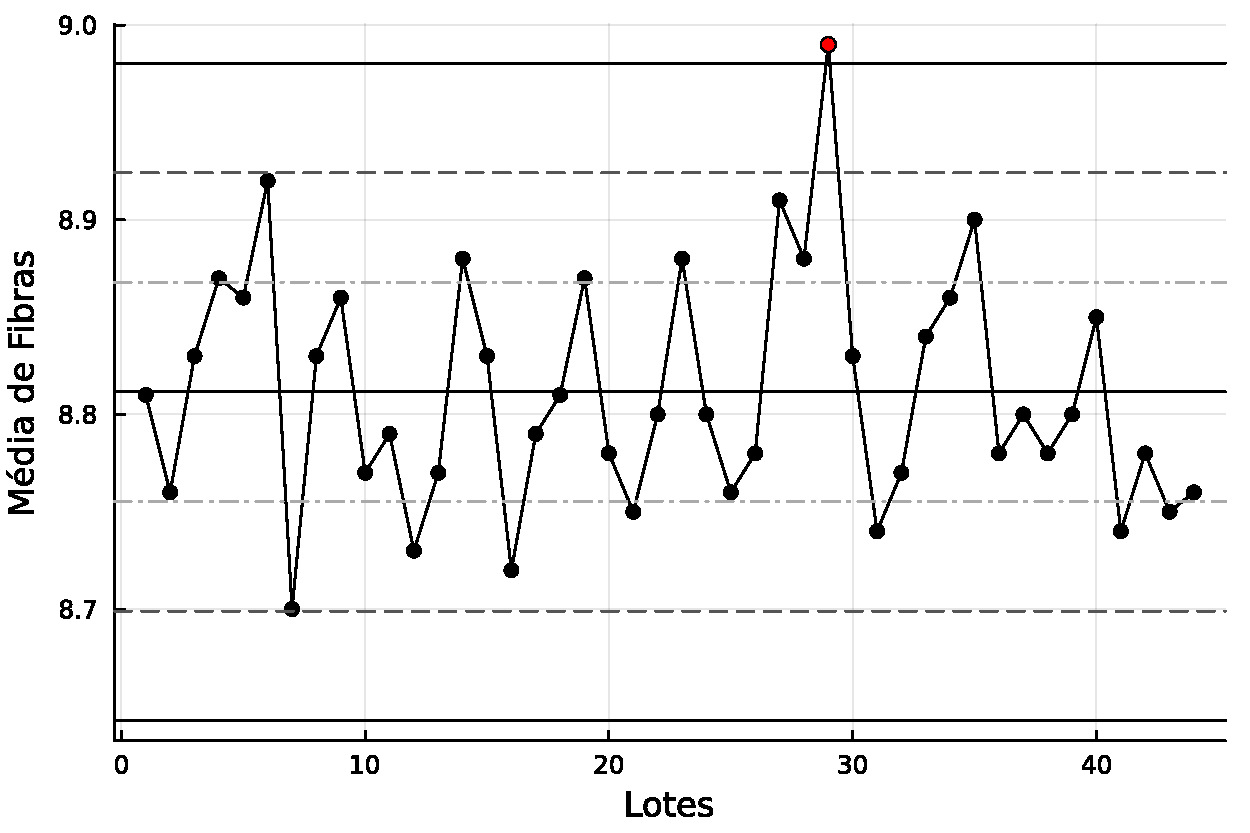
\includegraphics{relatorio_files/figure-pdf/fig-1-J1.pdf}

}

\caption{\label{fig-1}Gráfico de controle para observações individuais
da média de fibras em um lote.}

\end{figure}

\begin{figure}[H]

{\centering 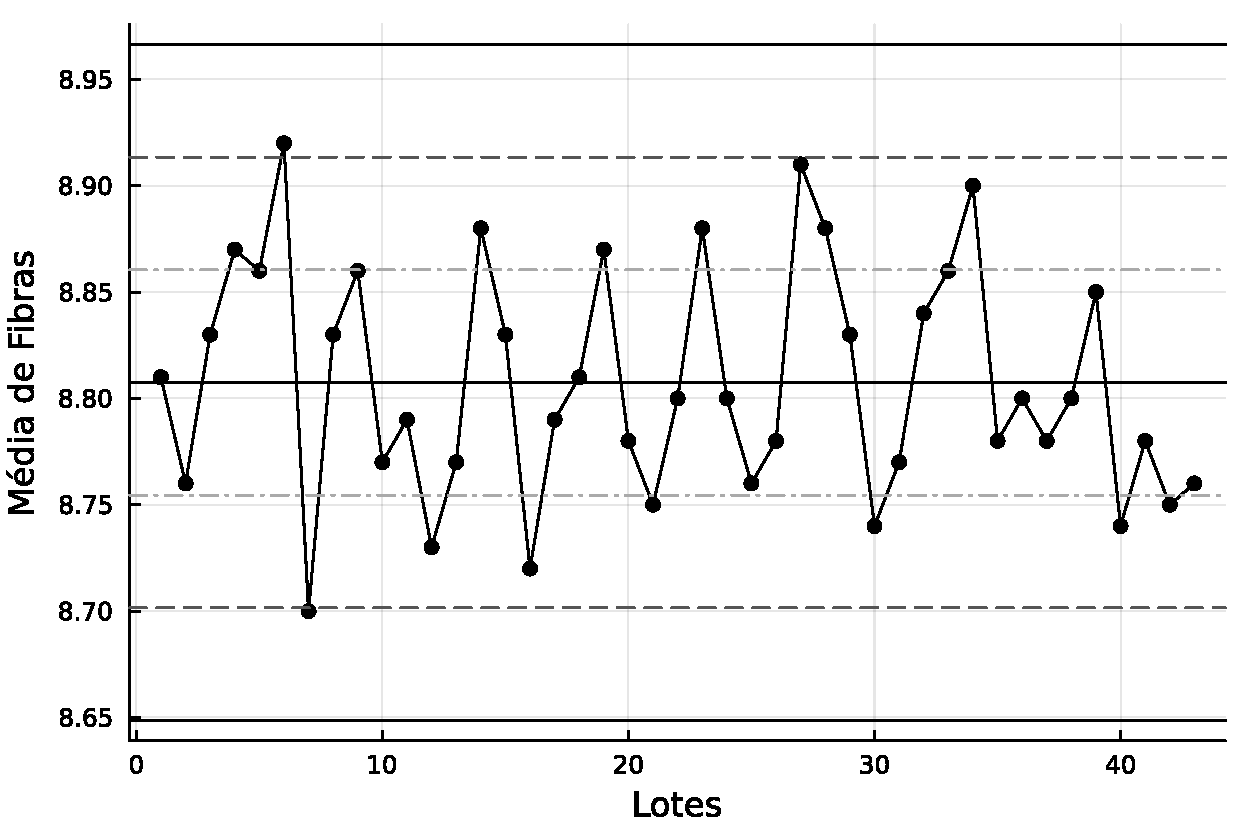
\includegraphics{relatorio_files/figure-pdf/fig-2-J1.pdf}

}

\caption{\label{fig-2}Gráfico de controle para observações individuais
da média de fibras em um lote com remoção de observações fora de
controle.}

\end{figure}

\hypertarget{amplitudes}{%
\subsubsection{Amplitudes}\label{amplitudes}}

A Figura~\ref{fig-3} e Figura~\ref{fig-4} tem-se os gráficos de
controles para amplitudes móveis. Na Figura~\ref{fig-3}, temos um ponto
fora de controle no lote 7, assim na Figura~\ref{fig-4} o gráfico foi
construído reconsiderando a média e o limite sem o ponto fora de
controle, semelhante ao que foi desenvolvido para Figura~\ref{fig-2}, a
Figura~\ref{fig-4} ficou como processo resultante, sem pontos fora de
controle e sem indícios de não aleatoriedade.

\begin{figure}[H]

{\centering 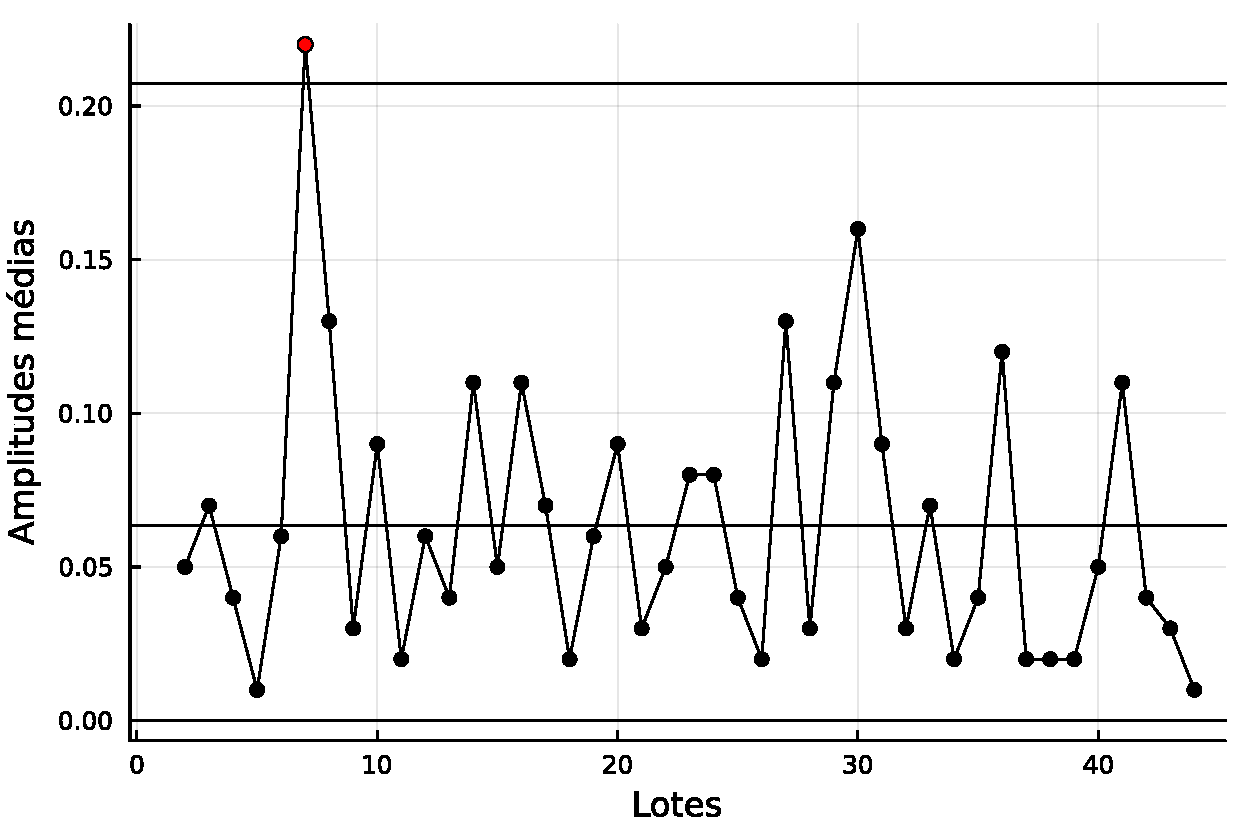
\includegraphics{relatorio_files/figure-pdf/fig-3-J1.pdf}

}

\caption{\label{fig-3}Gráfico de controle para amplitude móvies da
fibras.}

\end{figure}

\begin{figure}[H]

{\centering 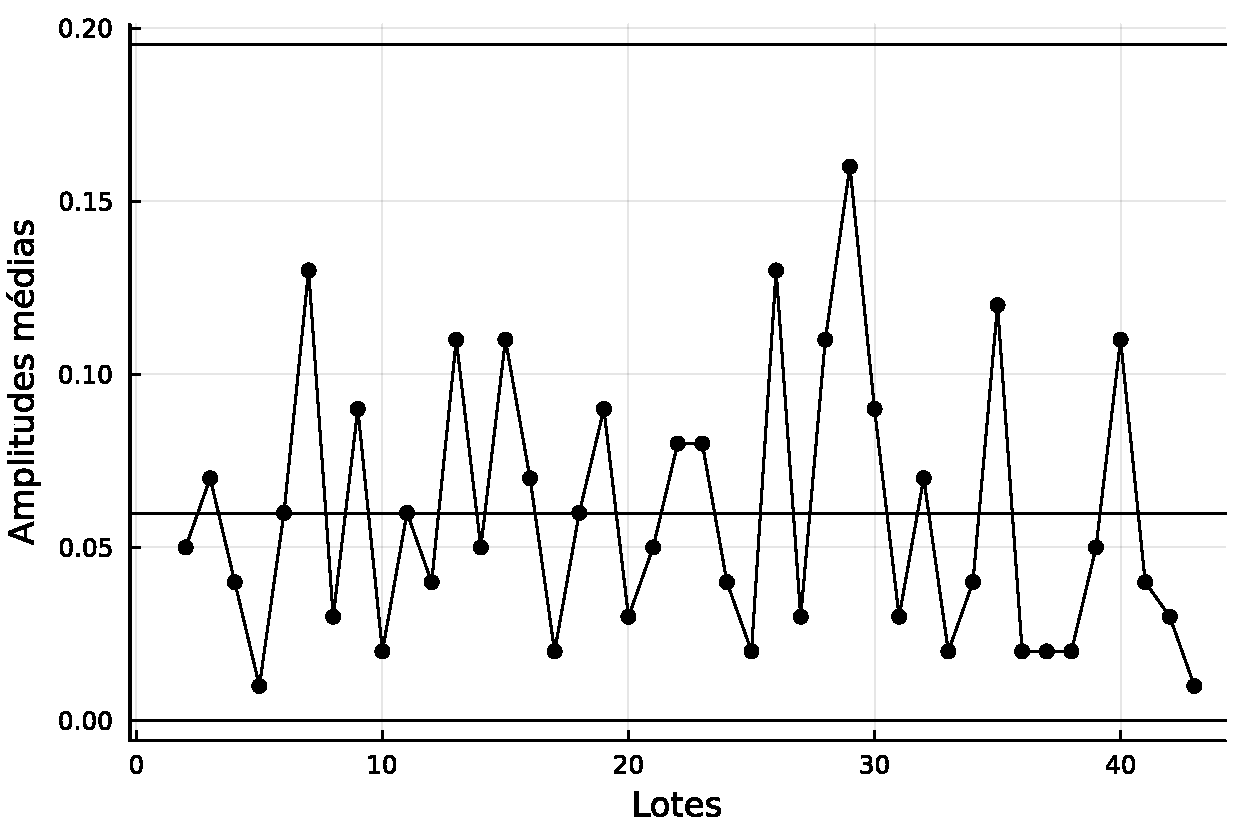
\includegraphics{relatorio_files/figure-pdf/fig-4-J1.pdf}

}

\caption{\label{fig-4}ráfico de controle para amplitude móvies da fibras
com remoção de pontos fora de controle.}

\end{figure}

\begin{verbatim}
1.1012363035098058
\end{verbatim}

\hypertarget{letra-b}{%
\subsection{Letra B}\label{letra-b}}

Avaliando \(C_p\) e \(C_{pk}\) em relação à capacidade do processo,
temos que:

\(C_p\) = \texttt{julia\ round(cp,\ digits\ =\ 4)}, é menor que 1.33,
assim temos evidência que o processo aceitável.

\(C_{pk}\) = \texttt{julia\ round(cpk,\ digits\ =\ 4)}, é menor que
1.33, assim temos evidência que o processo aceitável.

\hypertarget{exercuxedcio-2}{%
\section{Exercício 2}\label{exercuxedcio-2}}

\hypertarget{letra-a-1}{%
\subsection{Letra A}\label{letra-a-1}}

Na Figura~\ref{fig-5} temos o gráfico U para o número de artigos com
anomalia em um recipiente, seleciono-se o gráfico U, pois estamos
interassados no número de anomalias e não na proporção, outro fator para
não escolha de outros gráficos é o fato de as amostras serem
desbalanceadas (tamanho diferente). Assim também não foi verificado
nenhuma observação fora de controle e não há evidência de não
aleatoriedade.

\begin{figure}[H]

{\centering 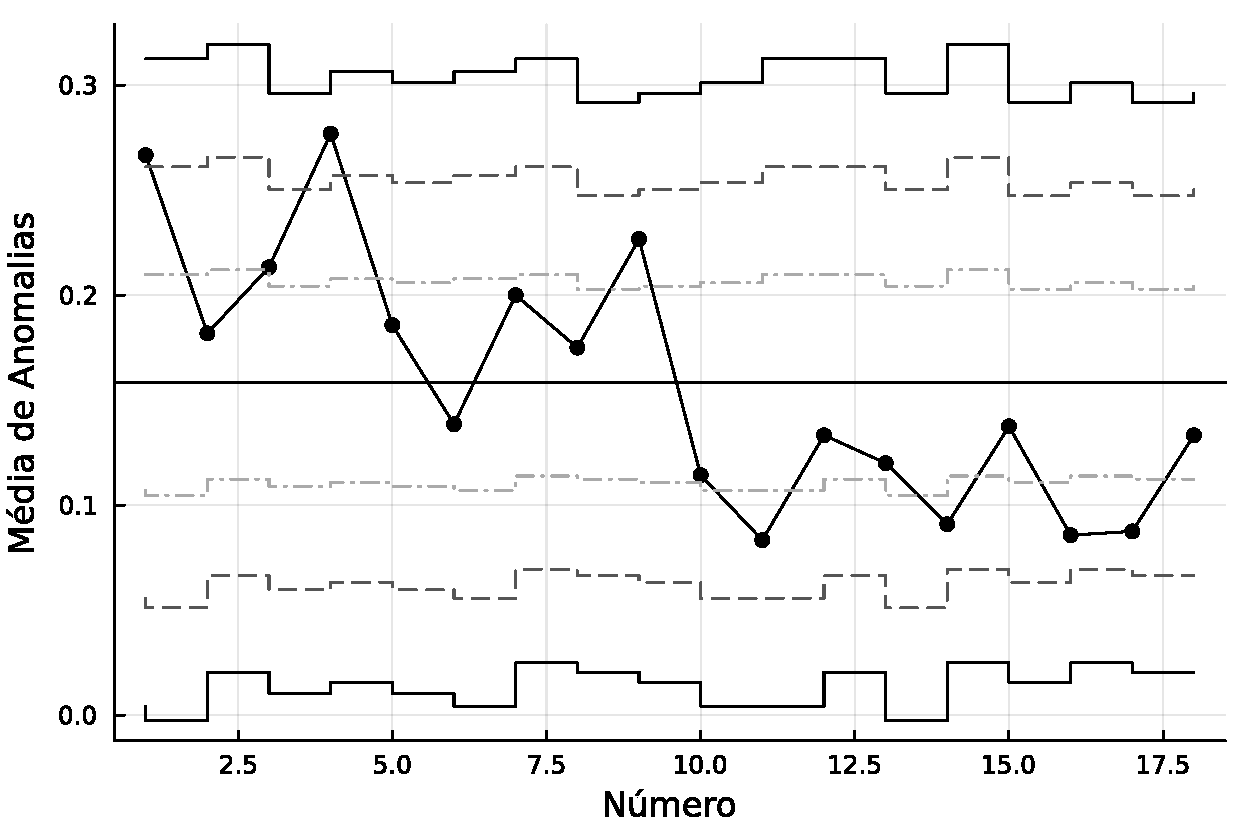
\includegraphics{relatorio_files/figure-pdf/fig-5-J1.pdf}

}

\caption{\label{fig-5}Gráfico de controle U para o número de artigos com
anomalia.}

\end{figure}

\hypertarget{letra-b-1}{%
\subsection{Letra B}\label{letra-b-1}}

Na Figura~\ref{fig-6} temos o gráfico U para o número de artigos com
anomalias não conformes em um recipiente. A justificativa para escolha
do gráfico U é a mesma para a Figura~\ref{fig-5}, estamos interassados
no número de anomalias e não na proporção, ainda temos amostras
desbalanceadas (tamanho diferente). Assim também não foi verificado
nenhuma observação fora de controle e não há evidência de não
aleatoriedade.

\begin{figure}[H]

{\centering 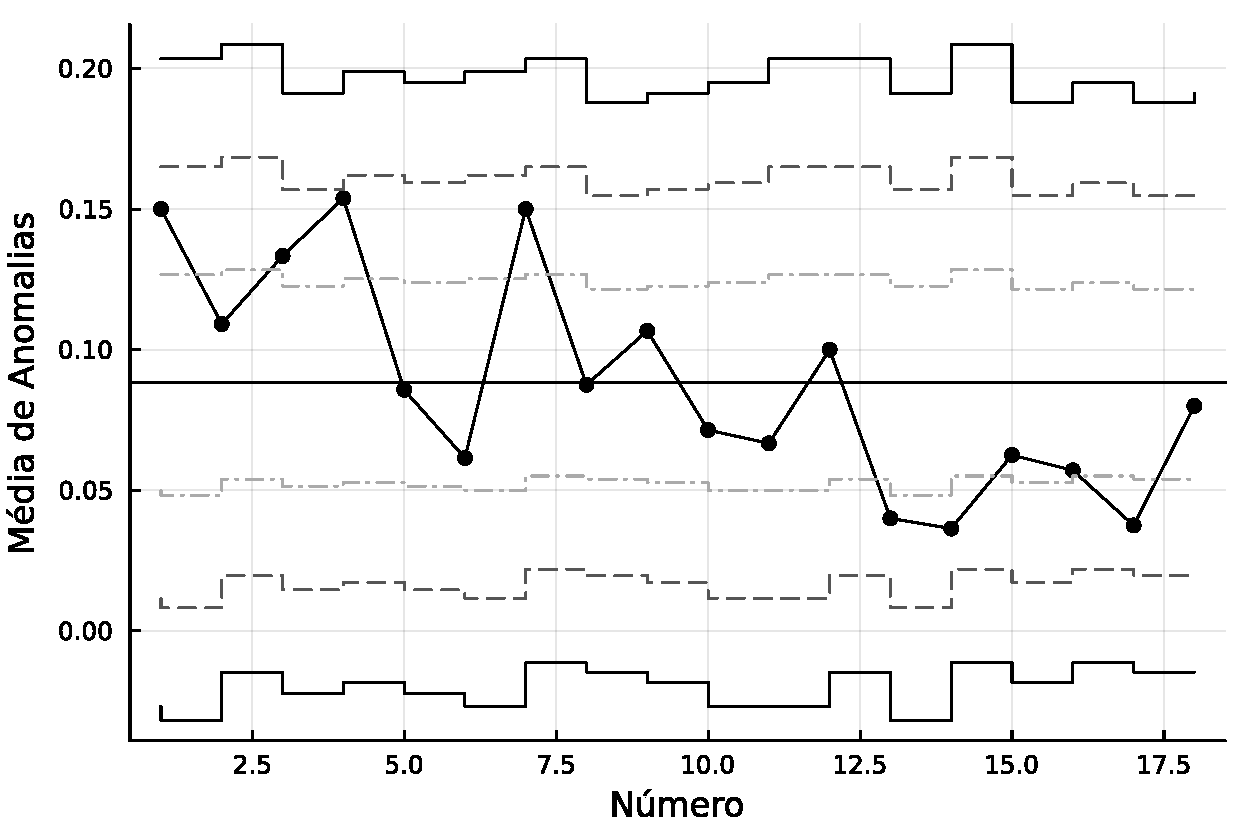
\includegraphics{relatorio_files/figure-pdf/fig-6-J1.pdf}

}

\caption{\label{fig-6}Gráfico de controle U para o número de artigos com
anomalias não conformes.}

\end{figure}



\end{document}
